\documentclass[10pt,twocolumn,letterpage]{article}
\usepackage{times,amsmath,amsfonts, bm, empheq, graphicx}
%\usepackage[dvips]{graphicx,graphics}
\usepackage{subfig}
\usepackage{titlesec}
\usepackage{float}
\usepackage{multirow}
\usepackage{url}

\titleformat{\section}{\Large\bfseries\filcenter}{\thesection.}{0.2em}{}
\titleformat{\subsection}{\large\bfseries\filright}{\thesubsection}{0.5em}{}
\titleformat{\subsubsection}{\normalsize\bfseries\filright}{\thesubsubsection}{0.5em}{}
\titlespacing{\section}{0pt}{3ex plus 0.5ex minus 0.2ex}{2ex plus .2ex}
\titlespacing{\subsubsection}{0pt}{2ex plus 0.1ex minus 0.1ex}{1ex plus .2ex}
\graphicspath{{figures/}}


% \titleformat{command}[shape]{format}{label}{sep}{beforecode}[aftercode]
% \fontsize{size}{baseline skip}

\setlength{\textheight}{8.5in} \setlength{\textwidth}{6.5in}
\setlength{\headheight}{0in} \setlength{\headsep}{0in}
\setlength{\parindent}{1pc}
\setlength{\parskip}{0pc}
\setlength{\oddsidemargin}{0in} 
\setlength{\evensidemargin}{0in}
\setlength{\columnsep}{1.5em}




\begin{document}
	\title{\textbf{Sentimental Analysis of IMDb Movie Reviews}}
	\author{Haoming Chen\\
		{\tt\small hchen549@wisc.edu}
		\and
		Ruiting Tong\\
		{\tt\small rtong5@wisc.edu}
		\and
		Dingyi Li\\
		{\tt\small dli283@wisc.edu}
	}
	\date{}
	\maketitle
	
	\section*{Abstract} 
	\textit{The objective of this project is to predict sentimental representation from the review of movies listed on IMDb via several classification machine learning algorithms. We collected 50,000 movie reviews and their sentiment scores (0 and 1) and processed them for analysis. The data are divided into 70\% of training set and 30\% of test set. Algorithms of SVM, KNN, Decision Tree, Logistic Regression, and Random Forest are trained and tested for accuracy. In particular, we used both the RBF and the linear kernels for SVM, and we applied bagging to Logistic Regression to obtain and verify an increased accuracy. As a result, we have found that the Logistic Regression is the best option for this task among others.} 			
	
	\section{Introduction} 
	With the Internet and modern technology, people are able to produce tons of text data every single day. We can find such data in emails, comments on articles, reviews on products, and social media, and there is a lot of information contained within such text data. When people write things down, they are motivated by certain emotions or attitudes. If they were happy with a product or an experience, they would compliment it and recommend it to others. If they had a terrible experience, they would criticize it and caution others. If we are able to organize and analyze the text data in a way that could accurately reflect users’ emotion or attitude, which is referred to as sentimental analysis, the companies could modify the service provided to each individual accordingly.
	
	Internet Movie Database (IMDb) is one of the most popular online databases for movies where millions of users read and write movie reviews. The users’ attitude toward one movie could be inferred by looking at the reviews they made. The objective of this project is to predict the sentimental
representation from the 50,000 review of movies listed on IMDb\cite{maas-EtAl:2011:ACL-HLT2011} via several classification machine learning models.In this project, we consider the simplest case where the sentiment is represented by a binary indicator: 1 meaning positive and 0 meaning negative. Despite such a simplification, it would be impossible for humans to read through millions of comments and reviews made by all movie watchers and label them each with a sentiment score. Therefore, it is necessary that we train and implement a machine learning algorithm to accomplish this task in our place. 
	
	Solving this classification problem is the first step to uncover the underlying habits of different users. One of the beneficiaries of such analysis would be streaming sites such as Netflix that need such data and methods to find out the movie types that particularly interest each user, and make accurate recommendations. On top of that, they can filter some junk ratings that are not conducive to helping others correctly understand and evaluate a movie, since they can be purely emotional and not based on reasons. 
	
	To find out the most suitable classification algorithm for this task, we experiment with SVM (RBF and linear kernels), KNN, Decision Tree, Random Forest, and Logistic Regression (with and without bagging). First of all, we extract 50,000 movie reviews and their corresponding 0-1 labels, and clean up the data by \textit{Natural Language Toolkit} (NLTK) package of Python. Then, we use 70\% of the data for training and the rest for testing. All the aforementioned algorithms are trained using the features selected in the first step. Lastly, test accuracy is computed for each algorithm, and further analyses such as McNemar's test and ROC comparisons are implemented to rank the algorithms.
	\section{Related work}
	Gautam, G. and Yadav, D conducted the sentiment analysis on the Twitter data and focused specifically on the extraction of adjectives within each document\cite{6897213}. They then progressed to several machine learning algorithms, including Naive Bayes, Support Vector Machine, and Maximum Entropy, followed by semantic analysis. The model performance was measured using precision, recall, and accuracy.
	
	Wilson et al’s work presented an approach to phrase-level sentiment analysis, which determines whether an expression is neutral or polar at first and then disambiguates the polarity of the polar expressions (Wilson, Wiebe, \& Hoffmann, 2005)\cite{wilson-etal-2005-recognizing}.  By considering prior polarity and contextual priority, they are able to identify negation and intensification on a phrase level and achieve much better results compared to the baseline model.
	
	Pang and Lee proposed a method to combine the traditional bag-of-words model with a minimum-cut framework to retain the polarity information\cite{DBLP:journals/corr/cs-CL-0409058}. Their approach will not only reduce computational complexity by reducing the length of texts but also achieve significantly better results compared to the model trained on the original full dataset. 
	
	However, the above researches focus more on extracting accurate and compact information from the raw data and limited to the use of a single machine learning model to improve prediction accuracy. Instead, this report will put a great emphasis on examining the power of ensembling methods in the case of natural language processing. We will extend on the previous machine learning models and combine them into a new model with different techniques.
	\section{Proposed Methods}
	\subsection{Support Vector Machine}
	Support Vector Machine (SVM) is a very commonly used algorithm for binary classification. The motivation behind it is relatively easy to understand. Basically, in an n-dimensional feature space, we want to find a (n-1)-dimensional hyperplane that separates the datapoints of two different classes, assuming that they are indeed separable by a line. Suppose that the hyperplane is $$\bm{\omega}^\top \bm{x} + b = 0.$$ and that \begin{equation}
	\bm{\omega}^\top \bm{x} + b = \pm1 \label{hyp}
	\end{equation} happen to be boundaries of the two classes that touch on at least one sample from each class respectively. Our goal is then to maximize the distance between the two hyperplanes in \ref{hyp}. Such a distance is given by $$\frac{2}{||\bm{\omega}||},$$ which can be interpreted as the distance between the two classes. The optimal hyperplane obtained from solving this maximization problem is used for prediction of new data. 
	
	So far, the idea of SVM has been introduced for the linear kernel. In fact, we can replace $\bm{x}$ in the constraint to an arbitrary function $\phi(\bm{x})$. Then the separating surface may no longer be a hyperplane. For example, a nonlinear kernel $\kappa(\bm{x},\bm{y}) = \phi(\bm{x})^\top \phi(\bm{y})$ that we have also employed is the Radial Basis Function (RBF), which is given by $$\kappa(\bm{x},\bm{y}) = \exp\left(-\frac{||\bm{x}-\bm{y}||^2}{2\sigma^2}\right),$$ where $||\cdot||$ denotes the Euclidean distance and $\sigma$ represents the bandwidth.  
	
	$L_1$ regularization is applied to SVM with linear kernel, and the coefficient $c$ is tuned. 
	\subsection{k Nearest Neighbors}
	$k$ Nearest Neighbors (KNN) is a classification algorithm whose training step only involves remembering the data. Suppose the size of the training set is $N$. In the fitting step, for each new sample $x^*$, the algorithm computes $$d_i = ||x^* - x_{\text{train},i}|| \text{ for } i = 1,2,...,N,$$ where $||\cdot||$ can be any distance function. Then we pick the $k$ indices from $\{1,2,...,N\}$ that are associated with the $k$ smallest distances. The predicted label for $x^*$ is the majority vote of the labels corresponding to these indices. 
	
	For our problem, we only consider the Euclidean distance, and $k$ is the only parameter we need to tune for. Considering that the optimal $k$ could be very large given a very high-dimensional data set, we search for such $k$ manually by narrowing down the search range.
	\subsection{Decision Tree}
	A decision tree predicts the label of a new sample by searching for the leaf node it belongs to. A tree can be either binary or non-binary, the information criterion for splitting a node can be "Gini", "Entropy", and so on, and the maximum depth is yet another hyperparameter that is set to prevent overfitting. In our project, we require the tree to be binary, while letting information criterion and maximum depth be unknown hyperparameters to optimize. Similar to the $k$ in $k$ Nearest Neighbors algorithm, the maximum depth is not searched for exhaustively. It is pinpointed by manually narrowing the search range.
	\subsection{Random Forest}
	Random Forest is an ensemble method augmented from decision trees. In our case, 100 trees are being trained, and at each node, a random set of features are chosen for the purpose of splitting. The prediction is the majority vote of the 100 trees. Notice that we do not perform any hyperparameter tuning for random forest for the sake of runtime. The maximum depth is set to "None" and the criterion is fixed as "Entropy".
	\subsection{Logistic Regression}
	Unlike the previous algorithms, the logistic regression is a soft classifier that predicts the conditional probability of a label being 0 or 1. Explicitly, 
	$$P(y = 0) = \frac{1}{1+\exp(\bm{\beta^\top}\bm{x})},$$ where $\bm{\beta}$ is estimated from the training set by minimizing \begin{align*}
	&-2\log L(\bm{X_1},...,\bm{X_N}) \\
	&= -2\log (\prod_{i=1}^{N}P_i^{1-Y_i}(1-P_i)^{Y_i})\\
	&= -2\sum_{i=1}^{N}(Y_i\bm{\beta}^\top\bm{X_i} - \log(1+\exp(\bm{\beta}^\top\bm{X_i}))).
	\end{align*} 
	However, in order to avoid overfitting, we add an $L_1$ regularization term to the cost function. Its coefficient is $c$, which is a hyperparameter we need to optimize.
	\subsection{Bagging}
	Bagging is an ensemble method to improve the performance of an algorithm. In our project, we only apply it to the logistic regression. This seemingly arbitrary decision is made not only because the logistic regression has a high test accuracy to be worthy of a further uplift, but also because it is the fastest algorithm among others so as to make bagging very applicable. The $L_1$ regularization coefficient is inherited from the regular logistic regression. 
	
	Different bagging sizes are attempted to help us visualize a pattern of increase in test accuracy. 
	\section{Experiment}	
	\subsection{Dataset}
	This dataset, originally obtained from IMDb database, is now published on Kaggle after initial preprocessing. The dataset provides a perfectly balanced class between positive and negative reviews, 25000 reviews for each label, 50000 reviews in total. The original movie rating is on a scale from 1 to 10. When the dataset was first processed by previous researchers, there was a threshold where a review will be labeled as negative when the rating is lower than 4 and positive when the rating is higher than 7. Though the dataset has been preprocessed, there are still some clean up work need to be done for our analysis.
	\subsection{Language Processing}
	\subsubsection{Removing HTML tags, special characters, and stop words}
	Being read the internet, raw review data contains tags that constitute the grammar of HTML, punctuation, and words that are not related to sentiments (stop words). We remove these irrelevant components: 
	
	\begin{figure}[H]
		\textsf{Before:}
		
		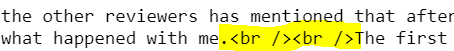
\includegraphics[width = \columnwidth]{html_tag}
		\textsf{After:}
		
		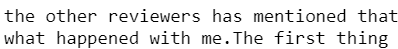
\includegraphics[width = \columnwidth]{html_tag_removed}
		\caption{Removal of HTML tags}
	\end{figure}
	
	\begin{figure}[H]
		\textsf{Before:}
		
		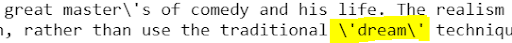
\includegraphics[width = \columnwidth]{special_char}
		\textsf{After:}
		
		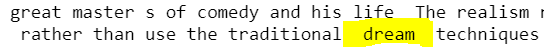
\includegraphics[width = \columnwidth]{special_char_removed}
		\caption{Removal of special characters}
	\end{figure}
	
	\begin{figure}[H]
		\textsf{Before:}
		
		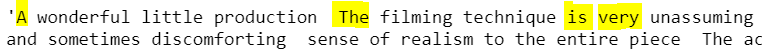
\includegraphics[width = \columnwidth]{stop_words}
		\textsf{After:}
		
		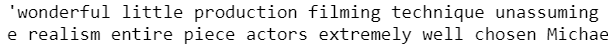
\includegraphics[width = \columnwidth]{stop_words_removed}
		\caption{Removal of stop words}
	\end{figure}
	\subsubsection{Text Stemming}
	Words such as "go" and "went" do not make essential difference. They are only different due to the English grammar. We therefore stem the text to coerce such words into one and the same feature:
	\begin{figure}[H]
		\textsf{Before:}
		
		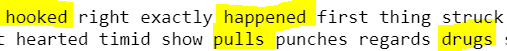
\includegraphics[width = \columnwidth]{stem}
		\textsf{After:}
		
		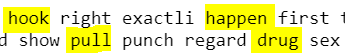
\includegraphics[width = \columnwidth]{after_stem}
		\caption{Text Stemming}
	\end{figure}
	
	\subsubsection{Vectorization}
	Now we need to turn features (words) into a design matrix. This step is performed by the \texttt{CountVectorizer} class imported from scikit-learn\ref{??}. A total of 70847 features are extracted.
	\begin{figure}[H]
		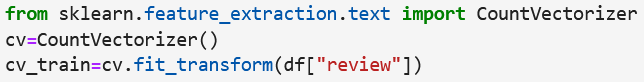
\includegraphics[width = \columnwidth]{vectorization}
		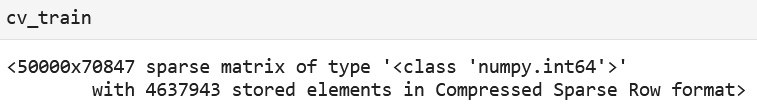
\includegraphics[width = \columnwidth]{vec_result}
		\caption{The code and result for vectorizing reviews}
	\end{figure}
	
	\subsection{Model Training}
	The dataset is divided into 70\% of training data and 30\% of test data. The split is stratified by the labels to guarantee that the training and the test sets contain homogeneous features. A random seed of 1 is used whenever randomness is involved. Hyperparameter tuning, when there are hypermarameters in an algorithm, is conducted by cross validation with k set to 5. 
	\subsubsection{SVM with RBF kernel}
	\subsubsection{KNN}
	We did not brute force through every possible k in parameter tunning process due to the harware limitation. As we can see from Figure 6, we first examined k from 50 to 300 by a step of 50. Then we narrowed our range down to around 200, and eventually achieved optimal k of 182.
		\begin{figure}[htbp]
			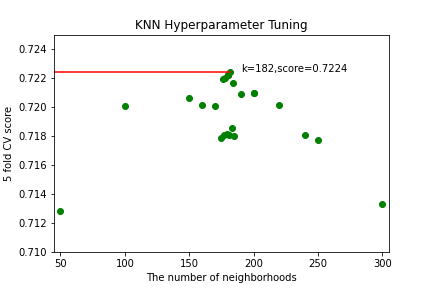
\includegraphics[width=\columnwidth]{KNN_hyper_tune}
			\caption{KNN Hypertunning}\label{KNN_hyper_tune}
		\end{figure}
	\section{Results}
	Table \ref{results} is a summary of the results obtained from each model. 
	\begin{table}[H]
		\begin{tabular}{|c|c|c|}
			\hline
			Model & Hyperparameter & Accuracy\\
			\hline 
			\hline
			SVM (RBF kernel) & NAN & 0.87947\\
			\hline
			SVM (Linear kernel) & C=0.01 & 0.88813\\
			\hline
			KNN (L2 Norm) & k = 182 & 0.72893\\
			\hline
			\multirow{2}{*}{Decision Tree}  & \small{max\_depth = 18} & \multirow{2}{*}{0.74087}\\
			                                 & \small{criterion = ‘gini’} & \\
			\hline
			\multirow{2}{*}{Random Forest} & \small{max\_depth = None} & \multirow{2}{*}{0.85853}\\
			 & \small{criterion = ‘entropy’}& \\
			\hline
			Logistic Regression & C=0.1 & 0.88967\\
			\hline
			Logistic Regression & \multirow{2}{*}{C=0.1(inherited)} & 0.89167 \\
			with Bagging & & (size = 60)\\
			\hline		
		\end{tabular}
		\caption{Test Accuracies and Hyperparameters for each Model}\label{results}
	\end{table}
	\subsection{SVM}
		The SVM model with RBF kernel achieves a test accuracy of 87.95\%, which is slightly less than the one with linear kernel, whose score is 88.82\%. However, for our problem, the training time of SVM with RBF kernel can take over an hour while linear SVM, even coupled with hyperparameter tuning, takes just a few minutes. We also compare these two methods by ROC curves and McNemar's Test. From Figure \ref{ROC_SVM}, we can see that the rendered ROC curve for linear SVM is above that of SVM with RBF kernel for a large portion of [0,1] but not completely.  
		\begin{figure}[htbp]
			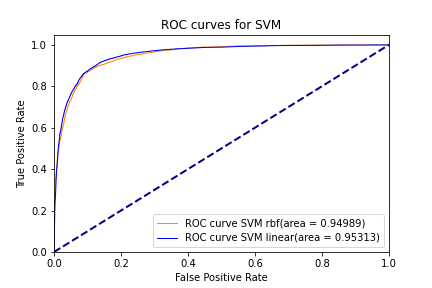
\includegraphics[width=\columnwidth]{ROC_SVM}
			\caption{Comparison of SVM models with rbf and linear kernels}\label{ROC_SVM}
		\end{figure} 
	
		The difference of performance in the models can also be detected by McNemar's test.  We set the significance level to $0.05$, and from Figure \ref{McNemar_SVM}, the McNemar's test statistic is $$\chi^2_{1} = \frac{(|556-426|-1)^2}{426+556} = 16.946,$$ whose associated p-value is $3.845827e-05 < 0.05$. While the test results indicates a significant difference, notice that we did not add a regularization term for SVM with RBF kernel. Adding it could possibly reduce overfitting and improve the performance. Yet considering an enormous amount of runtime needed for training this model, linear SVM is arguably better. 
		\begin{figure}[htbp]
			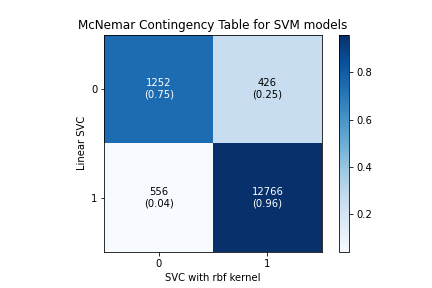
\includegraphics[width=\columnwidth]{McNemar_SVM}
			\caption{McNemar's Test}\label{McNemar_SVM}
		\end{figure} 
		\subsection{KNN}
		The KNN model achieves 72.89\% accuracy with optimal k of 182, which is the lowest accuracy achieved among all models we fitted in the project. The result is not surprising as we expected KNN to serve as a baseline model for comparison in our project because of its simplicity. Though it is possible that we did not find the best parameter value because of the interval search process we used, it is not worthy of going further on KNN since we are not expecting a dramatic improvement on accuracy caused by parameter value change.
		\subsection{Decision Tree \& Random Forest}
		The Decision Tree model achieves a test accuracy of 74.09\% while Randomn Forest achieves a test accuracy of 85.85\%. The result is not surprsing as Random Forest is an ensemble method that leveragges the power of multiple decision trees for making decisions.The performance can be illustrated with Figure 9, from which we can see that the ROC curve for Random Forest is much futhur above Decision Tree. 
		\begin{figure}[htbp]
			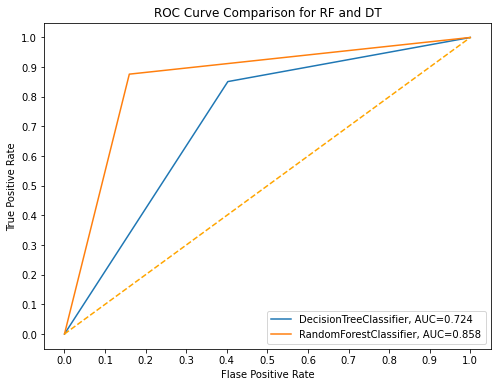
\includegraphics[width=\columnwidth]{ROC_RF_DT}
			\caption{Comparison of Decision Tree and Random Forest}\label{ROC_RF_DT}
		\end{figure} 
		The disadvantage of using Random Forest over Decision Tree is the overwhelming computional complexity.The parameter tunning process for Random Forest generally takes hours to run given a few specified parameter. However, considering the dramatic performance improvement, Random Forest is undoubtedly peferred over Decision Tree.
		\subsection{Logistic Regression}
		The Logistic Regression achieves a test accuracy of 88.97\%, which is the highest accuracy among all the models we have discussed so far. To see if we can furthur improve Logistic Regression performance, we applied bagging to it. We have changed the bagging size from 10 to 80 by a step of 10,fit the model, test on the testing set and record the accuracy. From Figure 10, we observe an overall improvement on accuracy and the highest accuracy, 89.17\%, is achieved at bagging size of 60.
		\begin{figure}[htbp]
			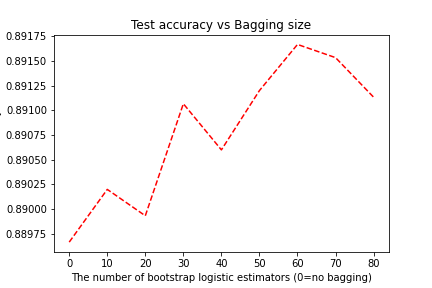
\includegraphics[width=\columnwidth]{Logistic_bagging}
			\caption{Test Accuracy vs Bagging Size}\label{Logistic_bagging}
		\end{figure} 	
		 Furthurmore, by plotting ROC curves for logistic regression with and without bagging in Figure 11, we can see that ROC curve with bagging lies entirely above the one without bagging. Therefore, we can confirm the usefullness of the ensemble method of bagging on Logistic Regression.
		
		\begin{figure}[htbp]
			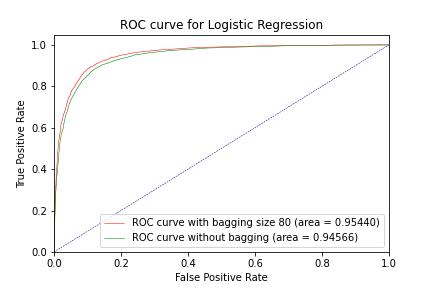
\includegraphics[width=\columnwidth]{ROCComparsion}
			\caption{ROC curve for Logistic Regression}\label{ROCComparsion}
		\end{figure} 	
	\section{Discussion}
	It is important to note that the performance of each model varies significantly from each other. KNN and Decision Tree turn out to perform the worst with 72.893\% and 74.08\% over all accuracy, which is much less accurate than the other 5 models. We conclude that KNN and Decision tree is not suitable for sentimental analysis. 

	However, we were expecting Random Forest to outperform other fitted models while it turns out to be the least accurate model excluding KNN and Decision Tree. It is possible that we did not find the best parameter for Random Forest. The reason is that Random Forest is computationally expensive.The grid search process took hours to run even though only a few parameter values were specified. Therefore, is it likely that the selected parameter value in our model is not the best. We are curious to see the performance of Random Forest if we are able to find the best parameter values with either a enhanced hardware or cloud computing.
	
\section{Conclusion}
	The analysis presented in the report aims to find the best algorithm for sentiment analysis of IMDb reviews. We demonstrated several potential algorithm including SVM, KNN, Decision Tree, Random Forest and Logistic Regression, train them on the same dataset with paramenter tunning and different machine learning techiniques, and evaluate the performance in terms of accuracy. We also use ROC curve, Confusion Matrix and Learning Curve as supplementary techniques to help us better evaluate and understand the fitted models.

	From Table 1, we cconclude that Logistic Regression performs the bestamong all fitted models, with an overall 89.167\% accuracy and Bagging size of 60. Nonetheless, it is possible that Random Forest could be improved during parameter tunning stage. Also, from the comparison of Logistic Regression with and without bagging, we conclude that bagging could help to improve the model accuracy.

	Finally, we hope our analysis lays a solid foundation for sentimental analysis. We hope our current analysis could be expand to Multi-label analysis since most of the rating system implemented in the business world is multi-lable. In the future, we hope more researchers could gather a dictionary will be helpful for organizations to effectively finish sentimental analysis on the collected reviews.

	

	\section{Contributions}
	Haoming Chen found the original dataset online and cleaned up the data for furthur analysis. Ruiting Tong coded the following models with parameter tunning: SVM(RBF kernel), Decision Tree, KNN and Logistic Regression with and with out bagging. Dingyi Li coded the rest models, SVM(Linear kernel) and Random Forest, and added code to generate confusion matrix, ROC curve and learning curve. Every one worked together and finished the project report.
	\section{Code}
	All of the code used to generate the plots and results for this project is on GitHub: \url{https://github.com/hchen549/stat451}

	\bibliographystyle{plain}	
	\bibliography{reference}
\end{document}